\section{Competing Applications}
\label{sec:competition}

With work and school continuing online, it is even more common to have multiple
applications simultaneously using the home network, potentially leading to
competition between any combination of VCAs, video streaming applications, or other popular
applications. In this section, we measure how VCAs perform in the presence of
other applications sharing the same bottleneck link. We focus on
link sharing with other VCAs, a single TCP flow (iPerf3), and two popular
video streaming applications, Netflix and YouTube (which uses QUIC).


\begin{figure}[t!]
\centering
\begin{subfigure}[t]{.4\textwidth}
    \centering
    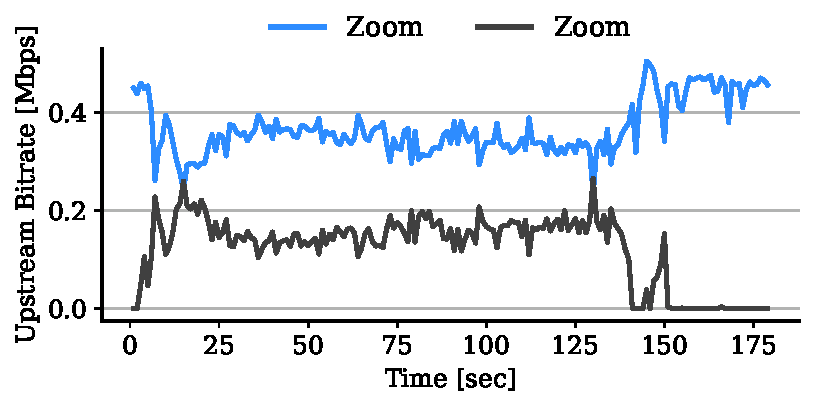
\includegraphics[width=1\textwidth]{figures/comp_ts/zoom_zoom_0.5_ul_r2.pdf}
    \caption{Zoom vs. Zoom}
    \label{subfig:zoom_zoom_0_5}
\end{subfigure}\hfill
\begin{subfigure}[t]{.4\textwidth}
    \centering
    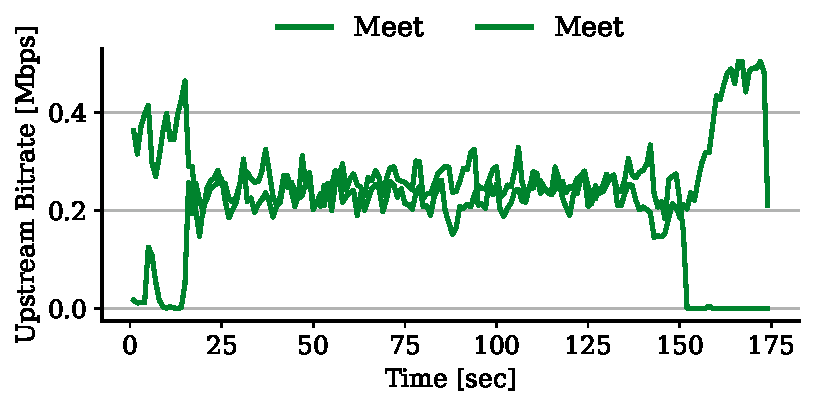
\includegraphics[width=1\textwidth]{figures/comp/meet_meet_0.5_ul_r1.pdf}
    \caption{Meet vs. Meet}
    \label{subfig:meet_meet_0_5}
\end{subfigure}
\caption{Upstream throughput of VCAs in competition on a 0.5~Mbps capacity link. Upper trendline is incumbent application and lower is competing application.}
\label{fig:meet-zoom-upld-0.5}
\end{figure}

\begin{figure*}[t!]
\centering
\begin{subfigure}[t]{.33\textwidth}
    \centering
    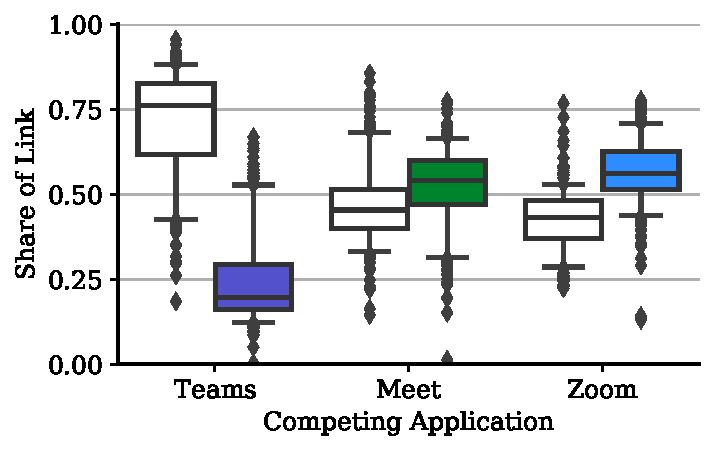
\includegraphics[width=1\textwidth]{figures/comp/box_plot_meet_dl_0.5_all.pdf}
    \caption{Meet}
    \label{fig:meet-dl-boxplot-0.5}
\end{subfigure}\hfill
\begin{subfigure}[t]{.33\textwidth}
    \centering
    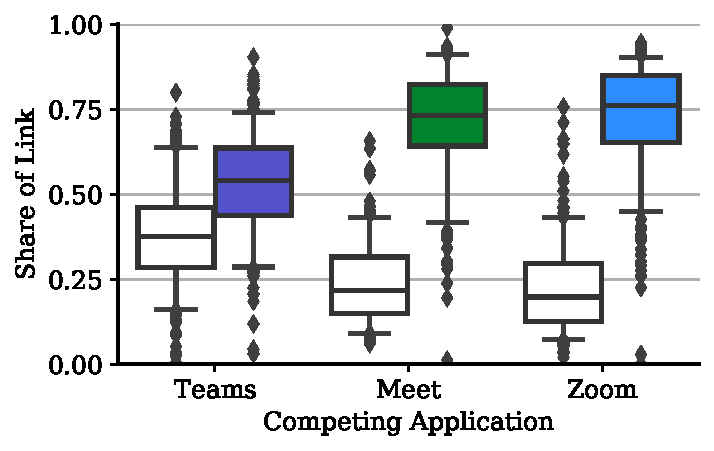
\includegraphics[width=1\textwidth]{figures/comp/box_plot_teams_dl_0.5_all.pdf}
    \caption{Teams}
    \label{fig:teams-dl-boxplot-0.5}
\end{subfigure}
\begin{subfigure}[t]{.33\textwidth}
    \centering
    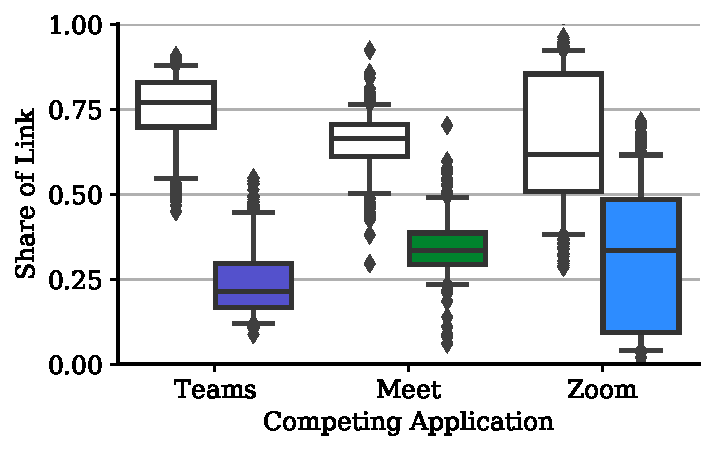
\includegraphics[width=1\textwidth]{figures/comp/box_plot_zoom_dl_0.5_all.pdf}
    \caption{Zoom}
    \label{fig:zoom-dl-boxplot-0.5}
\end{subfigure}
\caption{Downstream bitrate of applications in competition with each VCA on a 0.5~Mbps capacity link.}
\label{fig:dnld-boxplot}
\end{figure*}

\begin{figure}[t!]
\centering
\begin{subfigure}[t]{.5\textwidth}
    \centering
    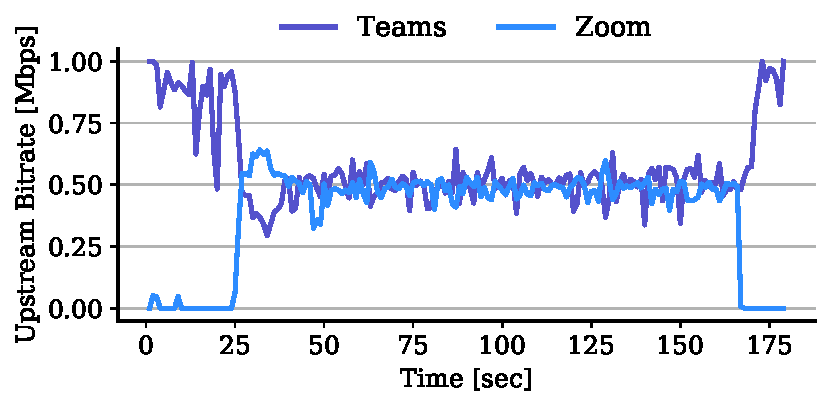
\includegraphics[width=0.8\textwidth]{figures/comp_ts/teams_zoom_1_ul_r2.pdf}
    \caption{Uplink}
    \label{fig:teams-zoom-up-1}
\end{subfigure}\hfill
\begin{subfigure}[t]{.5\textwidth}
    \centering
    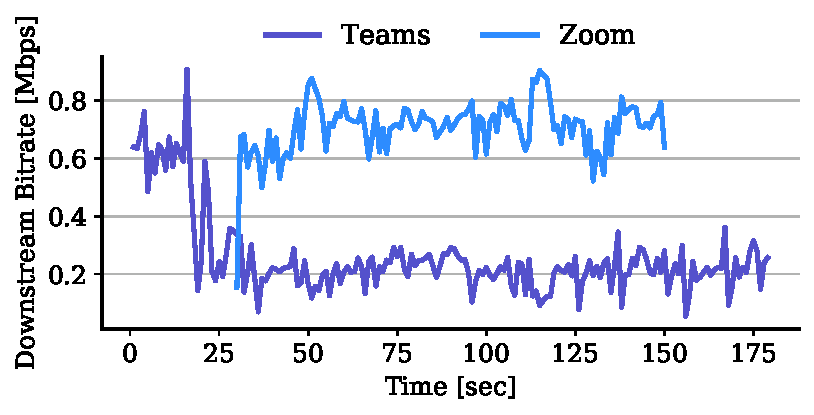
\includegraphics[width=0.8\textwidth]{figures/comp_ts/teams_zoom_1_dl_r2.pdf}
    \caption{Downlink}
    \label{fig:teams-zoom-down-1}
\end{subfigure}
\caption{Comparison of Teams competition behavior for uplink and downlink.}
\label{fig:teams-zoom-1}
\end{figure}


\noindent \textbf{Method}: As illustrated in Figure \ref{fig:competition-setup}, the setup for these experiments differs slightly from earlier ones. 
Instead of connecting the client directly to the router, the two matched clients, C1 and F1, are connected to the router via a switch. 
The link between the switch and the router is shaped by the router. For each test, C1 first establishes a VCA call with C2.
Approximately 30 seconds later, F1 initiates a competing application, which lasts for two minutes.
F1's counter-party, F2, depends on the type of competing application.
If the competing application is another VCA call, then F2 is another consumer laptop.
If the application is an iPerf3\footnote{The iPerf3 server uses TCP CUBIC and is  within the same network (average RTT ~2ms).} (TCP) flow, then F2 is a server on the same network,
  and if it is Netflix or Youtube, then F2 is a server for the respective service. Netflix and Youtube are launched directly in Chrome via \texttt{xdg-open}.
After the competing flow terminates, the incumbent flow continues for an additional minute.
We repeat each experiment 3 times, with bandwidth shaped symmetrically at levels of \{0.5, 1, 2, 3, 4, 5\}~Mbps.

\subsection{VCA vs. VCA}

VCAs can achieve their nominal bitrate when the link capacity is
4~Mbps or greater, which is expected because the link capacity exceeds the sum of
nominal bitrates of each VCAs. We then focus on the operating regime when the link
capacity is lower, leading to competition between the VCAs. 
With only two competing clients, we use the proportion of the link shared as a
metric to assess fairness. We call a VCA ``aggressive'' if it uses more than
half of the link capacity under competition, and ``passive'' otherwise.

Considering the upstream direction, we observe differences in how each VCA shares the
link. Figure~\ref{fig:boxplot-upld} shows a box plot of the upstream share of
an incumbent VCA and a competing VCA when the uplink capacity is 0.5~Mbps.  We
find that an incumbent Meet client shares the link fairly with a new Meet or
Teams client but backs off when a Zoom client joins (see
Figure~\ref{fig:meet_ul_box}). The results are similar for Teams except it
receives a slightly higher share while competing with Zoom compared to Meet.
Interestingly, Zoom is highly aggressive, both as an incumbent and a competing
application, using at least $75\%$ of the link capacity in the case it is an
incumbent client (see Figure~\ref{fig:zoom_ul_box}). In fact, Zoom's
congestion control is not even fair to itself.

Figure~\ref{subfig:zoom_zoom_0_5} illustrates this effect more clearly, with
the link sharing between two Zoom clients for a single experiment under
0.5~Mbps uplink capacity. We contrast this with the link sharing between two
Meet clients in Figure~\ref{subfig:meet_meet_0_5}, where both sessions converge to their
fair share of 0.25~Mbps. The results are similar for other uplink capacities,
with aggressive applications leaving more room for new clients if they achieve
their nominal bitrate.  

We find similar results for Zoom and Meet when downstream capacity is
constrained.
However, we find that Teams is passive when sharing downstream capacity, backing off to
all other VCAs, including other Teams flows. Figure~\ref{fig:teams-dl-boxplot-0.5} shows the
link share of an incumbent Teams client compared to the competing VCA under
0.5~Mbps downlink capacity. Teams achieves only 20\% of the link
when sharing with Meet and Zoom. We observe similar behavior for other downlink
capacities. Figure~\ref{fig:teams-zoom-down-1} illustrates how an incumbent
Teams client shares the link with a Zoom client at 1~Mbps downlink capacity.
Clearly the Teams client backs off to 0.2~Mbps. In contrast 
in the upstream direction, both Teams and Zoom converge to a near fair
share of the link, as shown in Figure~\ref{fig:teams-zoom-up-1}. 
Additionally, the downstream throughput in Figure~\ref{fig:teams-zoom-down-1} for Teams
degrades even before the Zoom call starts, likely because the
competing client opens the Zoom landing page to initiate a call. This can lead
to competing TCP traffic on the link and as we find in the next subsection,
Teams is extremely passive when competing against TCP. 


% The way each VCA shares the link with other applications is made clear in Figure \ref{fig:dnld-boxplot}. We see that Zoom uses well over $50\%$ of the available capacity against other VCA.

\begin{figure}[t!]
\centering
\begin{subfigure}[t]{.5\textwidth}
    \centering
    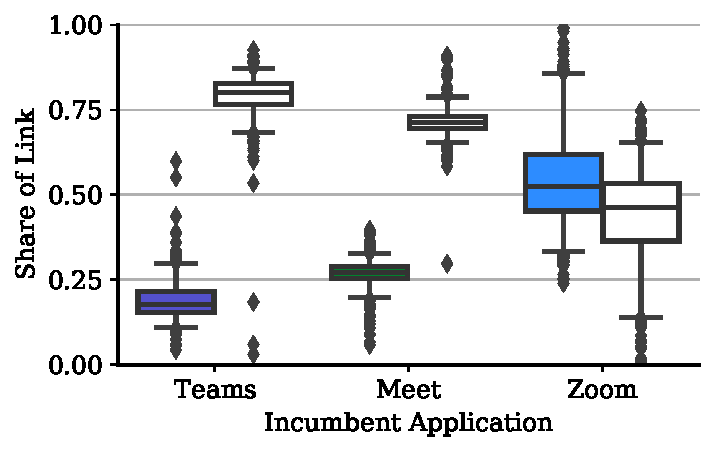
\includegraphics[width=0.7\textwidth]{figures/comp/box_plot_iperf_dl_2.0_all.pdf}
    \caption{Downlink}
    \label{subfig:boxplot-iperf-dl}
\end{subfigure}\hfill
\begin{subfigure}[t]{.5\textwidth}
    \centering
    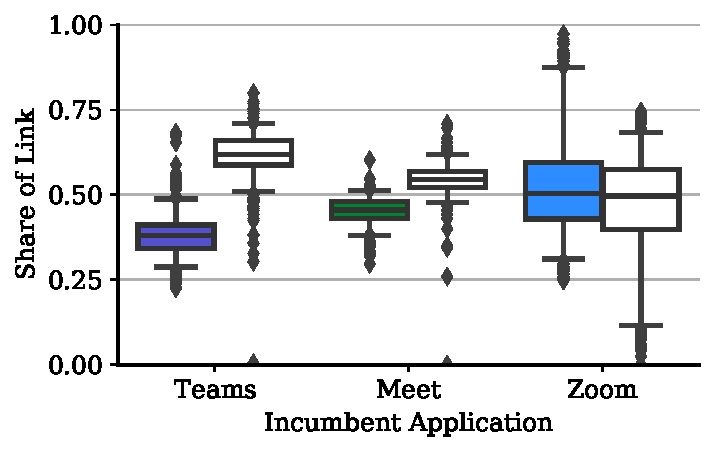
\includegraphics[width=0.7\textwidth]{figures/comp/box_plot_iperfup_ul_2.0_all.pdf}
    \caption{Uplink}
    \label{subfig:boxplot-iperf-ul}
\end{subfigure}
\caption{iPerf3 link sharing with VCAs on a 2~Mbps capacity link.}
\label{fig:boxplot-iperf}
\end{figure}

\begin{figure}[th]
    \centering
    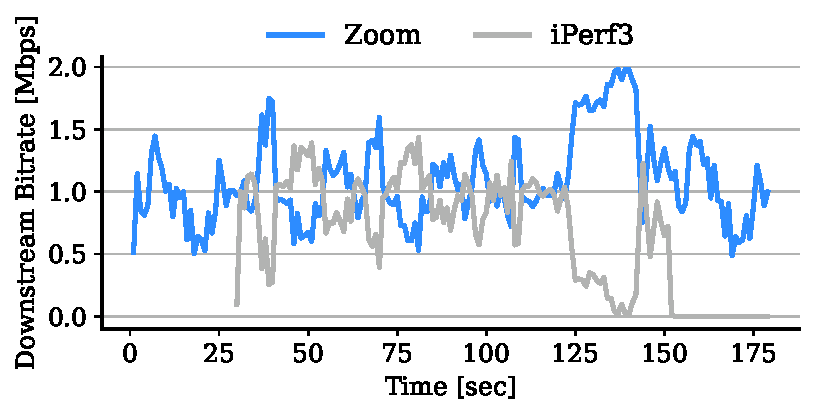
\includegraphics[width=\linewidth]{figures/comp_ts/zoom_iperf_2_dl_r3.pdf}
    \caption{Example of how Zoom probing can adversely affect competing applications}
	\label{fig:zoom-iperf-dl-2}
\end{figure}


\subsection{VCA vs. TCP}

We now compare how the three VCAs compete with a 120 seconds long TCP flow
from iPerf3. In a home network, a long TCP flow can be created by file
download or upload. We find that Zoom is highly aggressive,  especially at low
uplink and downlink capacity, consuming more than 75\% of the bandwidth under
a symmetric 0.5~Mbps link. Meet is TCP-friendly in the uplink direction but
not in the downlink, consuming $75\%$ of the bandwidth at 0.5~Mbps downlink
(figures omitted due to lack of space). Teams, on the other hand, is passive
and backs-off against a TCP flow in both upstream and downstream even at high
link capacity. Figure~\ref{subfig:boxplot-iperf-ul}
and~\ref{subfig:boxplot-iperf-dl} show how each VCA shares a 2~Mbps downlink
and uplink with iPerf3, respectively. Teams is able to use 37\% in uplink and
only 20\% in the downlink even at 2~Mbps. The low upstream throughput for
Teams with a TCP flow is particularly surprising as it was able to achieve its
fair-share when competing against (more aggressive) Meet and Zoom, as shown in Figure~\ref{subfig:teams_ul_box}). Meet and Teams achieve their nominal bitrate allowing iPerf3 to use rest of the link. Clearly, all the VCAs are not TCP CUBIC-friendly with Meet and Zoom being more aggressive and Teams being highly passive. 


\paragraph{Anomalous Zoom Bursts}: In the previous section, Figures \ref{fig:ts_upld} and \ref{fig:ts-dnld} showed how Zoom can send bursts of data for an extended period of time following a network disruption. Figure \ref{fig:zoom-iperf-dl-2} shows how this behavior is also exhibited when in competition with iPerf3. At about 125 seconds, Zoom's increased sending rate causes iPerf3 to abruptly lower its utilization. This confirms that the temporary bursts in Zoom, likely for inferring available bandwidth, can adversely affect other applications on a scare link. 


\begin{figure}[t!]
\centering
\begin{subfigure}[t]{.35\textwidth}
    \centering
    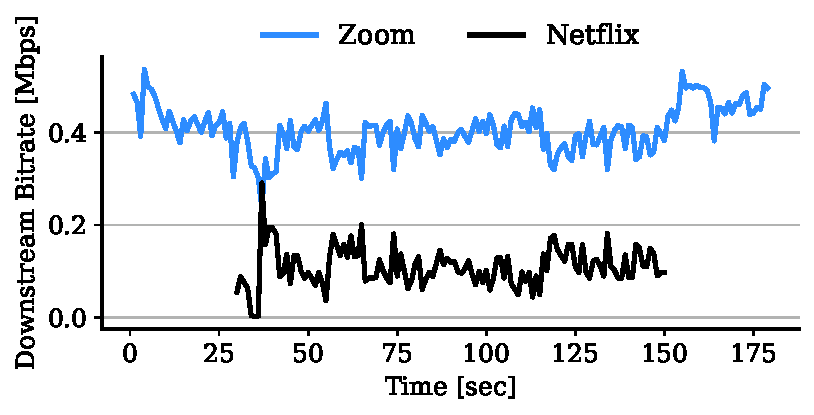
\includegraphics[width=1\textwidth]{figures/comp_ts/zoom_netflix_0.5_dl_r1.pdf}
    \caption{Downstream bitrate for Zoom and Netflix}
    \label{subfig:comp_zoom_netflix_bitrate}
\end{subfigure}\hfill
\begin{subfigure}[t]{.35\textwidth}
    \centering
    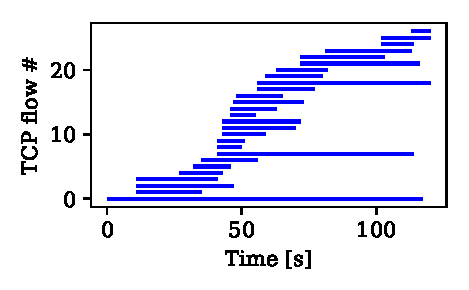
\includegraphics[width=1\textwidth]{figures/comp/netflix_connection_0_5.pdf}
    \caption{TCP connections opened by Netflix}
    \label{subfig:comp_netflix_conn}
\end{subfigure}
\caption{Netflix and Zoom competition on a 0.5~Mbps capacity link.}
\label{fig:comp_netflix_zoom}
\end{figure}

\subsection{VCA vs. Video Streaming}

We also compared each VCA's link share against two video streaming
applications, Netflix and YouTube,
which consume significant downstream bandwidth. 
YouTube uses QUIC, a UDP-based transport protocol,
which can be TCP-friendly under some configurations. 
Both Meet and Zoom are
very aggressive when competing against video streaming applications, using
over $75\%$ of the link capacity.In contrast, Teams uses
less than $25\%$ while competing with YouTube and Netflix at 0.5 Mbps.  
Figure~\ref{subfig:comp_zoom_netflix_bitrate} shows this effect, when a
Netflix client competes with an incumbent Zoom client at 0.5~Mbps downstream
capacity. , Zoom achieves an average throughput around 0.4~Mbps while
Netflix struggles to reach more than 0.1 Mbps. We observe this effect despite
the fact that Netflix is
known to using multiple TCP connections, especially when capacity is limited.
Figure~\ref{subfig:comp_netflix_conn} shows the TCP connections
opened by Netflix during the 120-second experiment. In total, Netflix opens 28
TCP connections, each with more than than 100 Kbits of data; at one point, it
opens 11 parallel TCP
connections. Despite this behavior, opening many TCP connections
does not improve link sharing for Netflix while competing with Zoom. 



